\documentclass[12pt]{article}

\usepackage[margin=1in]{geometry}
\usepackage{amsmath,amsthm,amssymb, graphicx, listings, minted}
\usepackage{placeins}

\lstset{language=Python}


% Janky stuff for figures below
\let\Oldsection\section
\renewcommand{\section}{\FloatBarrier\Oldsection}

\let\Oldsubsection\subsection
\renewcommand{\subsection}{\FloatBarrier\Oldsubsection}

\let\Oldsubsubsection\subsubsection
\renewcommand{\subsubsection}{\FloatBarrier\Oldsubsubsection}
% End of janky stuff 

\graphicspath{ {../images/} }

\begin{document}

\title{CSCE 633 Homework \#1}
\author{Jacob Fenger}
\date{\today}
\maketitle

\section*{Problem \#1}
\subsection*{a)}
To minimize the RSS, we must compute the partial derivatives of the RSS
function with respect to $w_0$ and $w_1$ respectively. This results in the
following two equations:

$$ \frac{\partial RSS(w_0, w_1)}{\partial w_0} = \sum_{n=1}^{N} 2(y_n - w_0 - w_{1}x_{n})(-1) $$
$$ \frac{\partial RSS(w_0, w_1)}{\partial w_1} = \sum_{n=1}^{N} 2(y_n - w_0 - w_{1}x_{n}(-x_{n})) $$

We can then solve the first equation for $w_0$. This is easily done by factoring
in the $-1$ and then splitting the summation up.

$$ \sum_{n=1}^{N} y_n = w_1 \sum_{n=1}^{N} x_n + N w_0 $$
$$ w_0 = \frac{1}{N} \sum_{n=1}^{N} y_n - w_1 \frac{1}{N} \sum_{n=1}^{N} x_n $$

Similarily, we can do the same for $w_1$:

$$ \sum_{n=1}^{N} x_n y_n = w_1 \sum_{n=1}^{N} x_{n}^{2} + w_0 \sum_{n=1}^{N} x_n $$

We then solve for $w_1$ by plugging in what we found for $w_0$.


$$ w_1 = \frac{\sum_{n=1}^{N} x_n y_n - N (\frac{1}{N}\sum_{n=1}^{N} x_n)(\frac{1}{N}\sum_{n=1}^{N}y_n)}
		{\sum_{n=1}^{N} x_{n}^{2} - N (\frac{1}{N} \sum_{n=1}^{N} x_n)^{2}} $$

\subsection*{b)}

We can use our previous solution for $w_0$ to replace all the $\sum_{n=1}^{N} x_n$ with $\bar{x}$
and similarily for $y_0$.

$$ w_0 = \bar{y} - w_1 \bar{x} $$

Solving for $w_1$ requires a trick or two in order to match the expression 
defined in the homework. We first can do all the replacements like we did for $w_0$:

$$ w_1 = \frac{\sum_{n=1}^{N} x_n y_n - N (\bar{x})(\bar{y})}{\sum_{n=1}^{N} x_{n}^{2} - N (\bar{x})^{2}} $$

Through a few tricks of adding and subtracting certain terms that is a bit tedious, we should
end up with:

$$ w_1 = \frac{\sum_{n=1}^{N}(x_i - \bar{x})(y_i - \bar{y})}{\sum_{n=1}^{N}(x_i - \bar{x})^{2}} $$

\subsection*{c)}

Both $\bar{x}$ and $\bar{y}$ represent the sample means for both populations. 
Additionally, $\sum_{n=1}^{N} (x_n - \bar{x})^{2}$ represent the total sample variation 
in sample $x$. The same can be said for $y$.

\section*{Problem \#2}

\subsection*{a)}

Let $\nabla J$ be the gradient vector and $H_J$ the Hessian Matrix of J evaluated at $w(k)$.

We can write the target function using the Taylor series expansion around $w(k)$ as the 
following:

$$ J(w) \approx J(w(k)) + (\nabla J|_{w=w(k)})^{T} \cdot (w-w(k)) + \frac{1}{2}(w-w(k))^{T} 
\cdot H_J|_{w=w(k)} \cdot (w-w(k)) $$

\subsection*{b)}

To solve this problem, we simply need to plug in $w(k) - \alpha(k) \cdot \nabla J|_{w=w(k)}$
for $w$ in the equation from a). 

$$ J(w(k+1)) \approx J(w(k)) + (\nabla J|_{w=w(k)})^{T} \cdot (-\alpha(k) \cdot \nabla J|_{w=w(k)})
+ \frac{1}{2}(-\alpha(k) \cdot J|_{w=w(k)})^{T} \cdot H_J|_{w=w(k)} \cdot (-\alpha(k) \cdot J|_{w=w(k)}) $$

$$ J(w(k+1)) \approx J(w(k)) - \alpha(k) \cdot \parallel{\nabla J|_{w=w(k)}}\parallel{}_{2}^{2} 
+ \frac{1}{2} \alpha(k)^{2} \cdot (\nabla J|_{w=w(k)})^{T} H_J|_{w=w(k)} (\nabla J|_{w=w(k)}) $$

\subsection*{c)}

For this problem, we can set $J(w) = 0$ and take the partial derivative with respect to $\alpha(k)$:

$$ \frac{\partial J}{\partial \alpha(k)} = 
- \parallel{\nabla J|_{w=w(k)}}\parallel{}_{2}^{2} + \nabla J|_{w=w(k)})^{T}H_J|_{w=w(k) 
\nabla J|_{w=w(k)}} \alpha(k) $$

Then solve for $\alpha(k)$:

$$ \alpha(k) = \frac{\parallel{\nabla J|_{w=w(k)}}\parallel{}_{2}^{2}}
{(\nabla J|_{w=w(k)})^{T} H_J|_{w=w(k)} (\nabla J|_{w=w(k)})} $$

\subsection*{d)}

Given the above expression, we must compute the gradient each iteration. 
Additionally we have to compute the second derivatives as well given we 
utilize the Hessian matrix. Overall, I would argue that the runtime $\Theta(n^3)$
for computational cost.

\section*{Problem \#3}

\subsection*{a)}

Below, you will find figures with explanations of what the graph consists of 
and what it may be able to tell us. 


\begin{figure}[!htb]
\begin{center}
  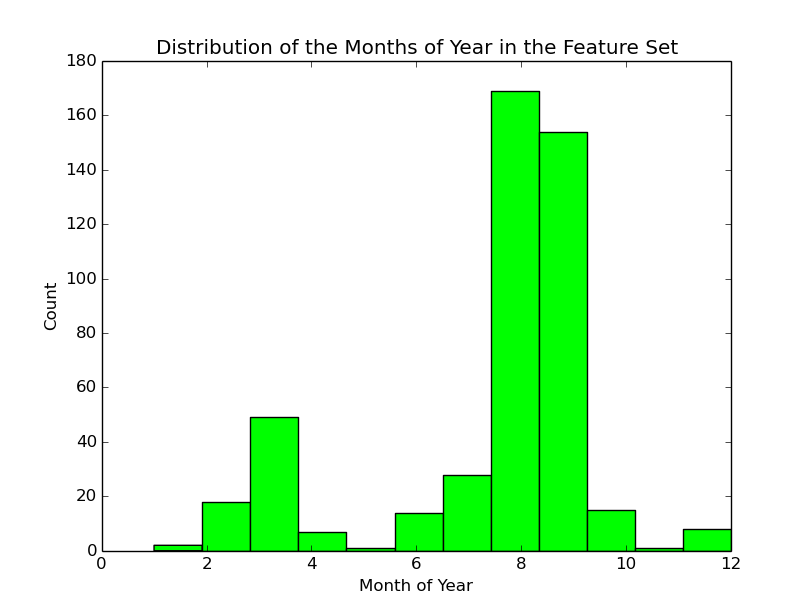
\includegraphics[scale=0.4]{month-distribution.png}
  \caption{Looking at the distributions of the months, a categorial variable.}
\end{center}
\end{figure}

\begin{figure}[!htb]
\begin{center}
  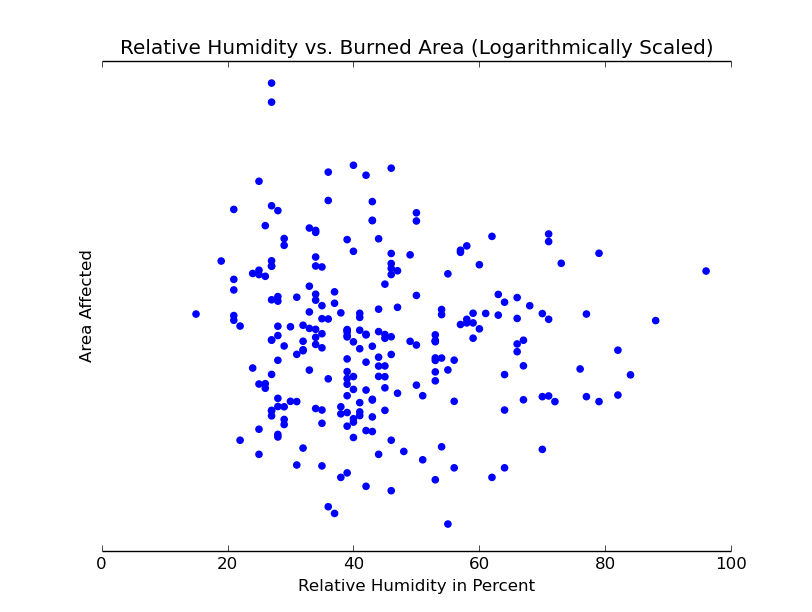
\includegraphics[scale=0.4]{humidity-area.png}
  \caption{A comparison of humidity in percent and the log of burned area.}
\end{center}
\end{figure}

\begin{figure}[!htb]
\begin{center}
  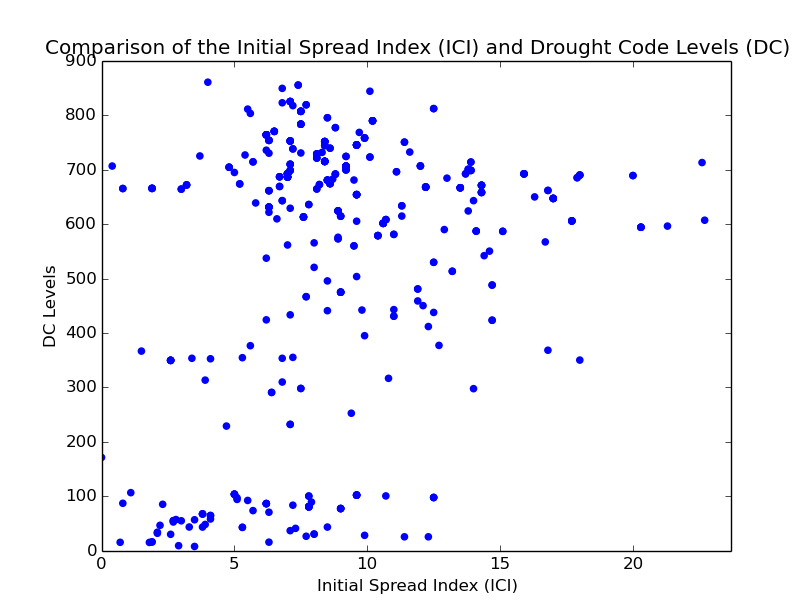
\includegraphics[scale=0.4]{ici-droughtcode.png}
  \caption{Comparison of the ICI and droughtcode. Not much of a correlation is visible.}
\end{center}
\end{figure}

\begin{figure}[!htb]
\begin{center}
  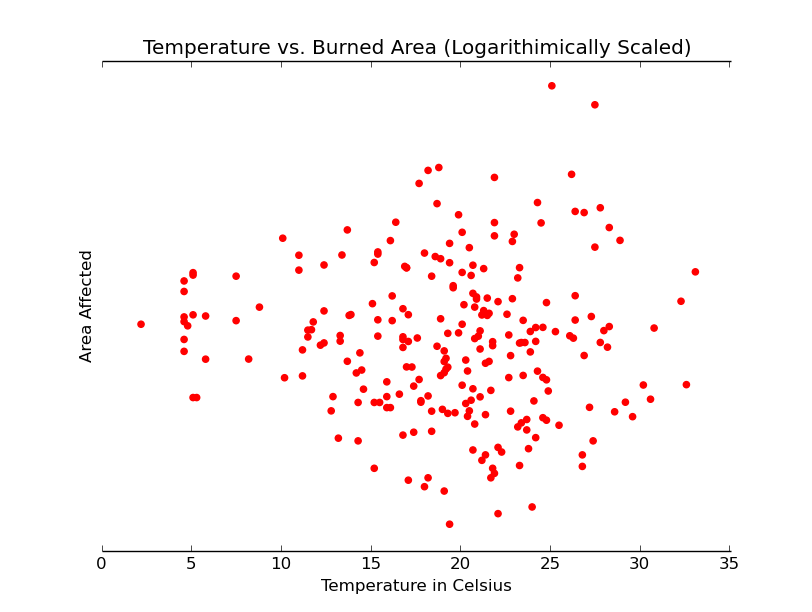
\includegraphics[scale=0.5]{temperature-area.png}
  \caption{A comparison of temperature and the corresponding burned area (Log scaled)}
\end{center}
\end{figure}

Categorical variables for this data set include: X, Y, month, and day.
Continuous features include: FFMC, DMC, DC, ISI, temp, RH, wind, rain, and area.

\subsection*{b)}
\textit{See code for dichotomization.}
	\subsubsection*{b.i)} 
	\textit{See code.}

	\subsubsection*{b.ii)}
	The best K values found using cross validation were: 3, 5, and 7. These had the lowest errors. 
	I utilized 10-fold cross validation to compute these values.
	\begin{figure}[!htb]
	\begin{center}
	  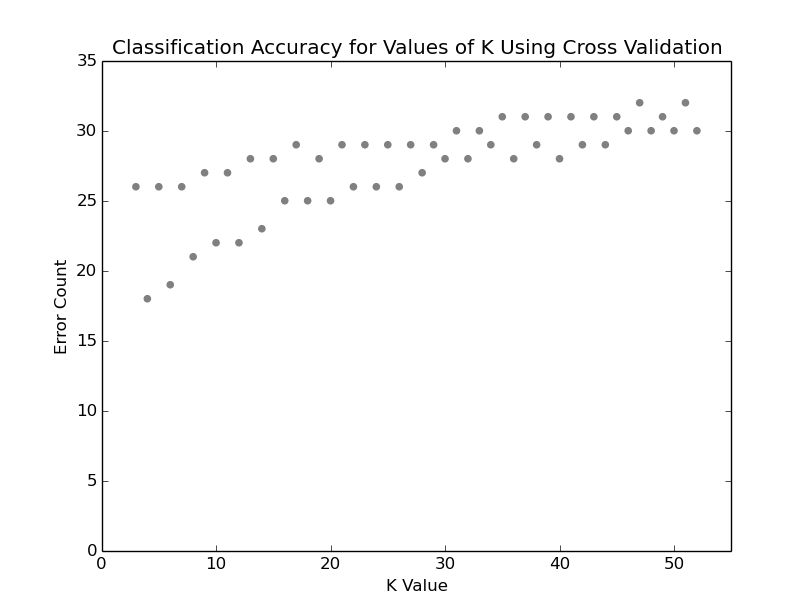
\includegraphics[scale=0.5]{k-value-error.png}
	  \caption{Number of errors corresponding to the K values when doing 10-fold cross validation.}
	\end{center}
	\end{figure}

	\subsection*{b.iii}
	For the test set, I used a value of $K=7$ since that was one of the better K values found 
	when doing cross validation. \textbf{The accuracy ended up being: $0.67\%$}.

\subsection*{c)}

	\subsubsection*{c.i)}
	The histograms of both the burned area and the logarithm of the burned are shown below:
	Notice that the log(area) graph depicts a normal distribution instead of being 
	skewed with a right tail in the first histogram.

	\begin{figure}[!htb]
	\begin{center}
	  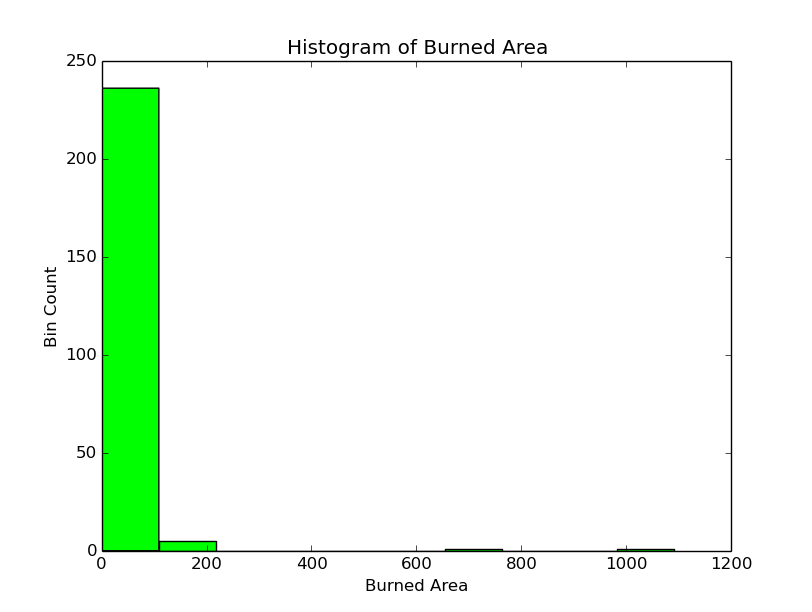
\includegraphics[scale=0.5]{histogram-burned.png}
	  \caption{Histogram of the burned area.}
	\end{center}
	\end{figure}

	\begin{figure}[!htb]
	\begin{center}
	  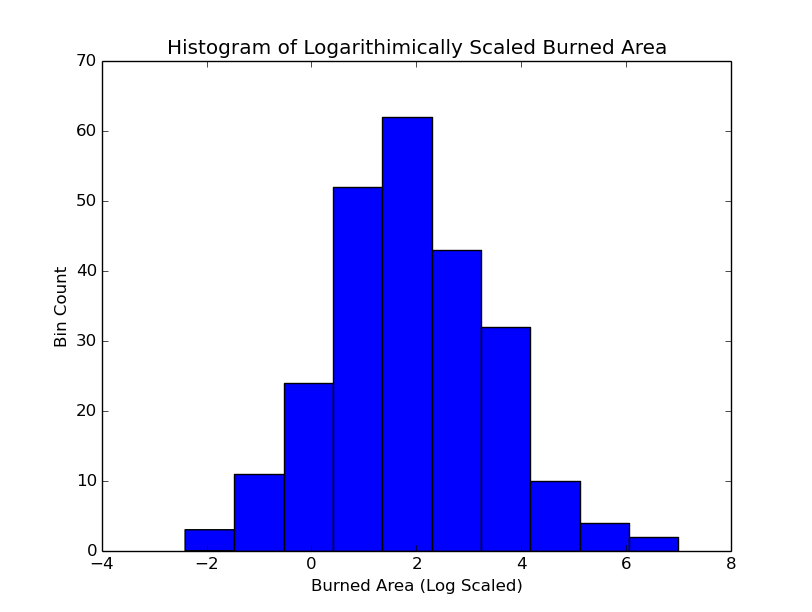
\includegraphics[scale=0.5]{log-histogram-burned.png}
	  \caption{Histogram of the logarithm of the burned area.}
	\end{center}
	\end{figure}

	\subsubsection*{c.ii)}
	\textit{See code.}

	\subsubsection*{c.iii)}
	The computed residual sum of squares error (RSS) was: \textbf{103808.628527}.

	A correlation coefficient of \textbf{0.1652} was found. This means that there
	was a very weak positive correlation. In other words, I am not confident that
	this method of prediction is very accurate.

	\subsubsection*{c.iv)}
	Taking the square of the input feature matrix yieled similar results
	with an RSS of \textbf{103023.35} and a correlation 
	coffecient of \textbf{0.1648}.

\section*{Code}

\subsection*{Main: }
\inputminted{python}{../main.py}

\subsection*{Inspection of Data:}
\inputminted{python}{../inspection.py}

\subsection*{KNN Functions:}
\inputminted{python}{../KNN.py}

\subsection*{Linear Regression Implementation:}
\inputminted{python}{../linear_regression.py}
\end{document}
